%#!platex --src-specials main.tex

\chapter{触覚情報の次元削減手法と\\機械学習}
\label{chap:method}
本章では,\ref{sec:prepro}にて加速度触覚データの分類に用いた3軸加速度データの前処理について記述する . \ref{sec:cnn}にて触覚情報分類に用いる畳み込みニューラルネットワークの概説を行う. 
\section{触覚情報の次元削減手法}
\label{sec:prepro}
次元削減を行った3軸加速度触覚データと次元削減を行わず正規化を施した3軸加速度触覚データ, 次元削減を行わず正規化も行わない3軸加速度触覚データのうち, どの取り扱い手法が分類に適しているかを調査するため, それぞれのアルゴリズムで前処理した加速度触覚データを作成した. 
対象としたデータは J. Kuchenbecker によって提案された DFT321 \cite{dft321} の論文中に比較検討対象として上がっていた5つのアルゴリズムによって次元削減された1軸の触覚データと, 各軸ごとに大きさを0から1の間で正規化した3軸加速度触覚データ, 何も施さない3軸加速度触覚データである. 前処理工程の末尾に付く321という文字は 3-dimensions to 1-dimension の略である. 
\subsection{比較対象アルゴリズム}
\subsubsection{Single - Axis : SA321}
SA321について説明する. これはセンサによって得られた3軸データのうち, 1軸のデータのみを抽出して扱う手法である. 
これについて, センサのx,y,z軸に対してそれぞれの信号を$SA321-x$, $SA321-y$, $SA321-z$とし3つの1軸データとして取り扱う.  
テスクチャに対しての鉛直方向や移動軸に対して分類を決定づける特徴がでると想定できるが, 単純にx,y,z軸に沿って現れるという保証はないため大幅な信号損失の可能性が問題となる.  

\subsubsection{Sum of Components : SoC321}
SoC321 について説明する. これは3軸加速度データの$x$,$y$,$z$成分を単純加算し, 1つの信号として扱う手法である. 3軸信号を$a(t)$とすると, 
\begin{equation}
SoC321(a)=a_{x}+a_{y}+a_{z} 
\end{equation}
計測するテクスチャに特徴的な振動があれば指自体が何かしらの挙動を起こし, 取り付けられた加速度センサも3軸同時に特徴的な振動を計測できるため, 3軸間の時間的相関は考えられる. 
ただし3軸加速度データを取り扱う上で, 正の向きや負の向きの加速度は軸が違えば単純に比較できないことは明白であるが, SoC321 において加速度を単純加算しているため, 正負の振動の情報に対して有意な値を保持することができない可能性がある. 

\subsubsection{Vector Magnitude : Mag321}
Mag321 について説明する.これは3軸加速度データの$x$,$y$,$z$成分に対してそれぞれ2乗し平方根をとったものを, 1つの信号として扱う手法である. 
\begin{equation}
Mag321(a)=\sqrt{{a_{x}}^2+{a_{y}}^2+{a_{z}}^2} 
\end{equation}
これは前述の正や負の加速度の向きを考慮せずベクトルの大きさのみに情報を絞って扱っているため, それぞれの軸の絶対的な振動のスケール情報は残る. しかしこれも正負の振動情報に対して有意な値が保持できない可能性がある.

\subsubsection{主成分分析 (Principal Component Analysis, PCA)}
主成分分析 (PCA) について概説する. これは代表的な次元圧縮方法であり, 以下の流れで計算を行う. 
\begin{enumerate}
  \item 全データの平均を求める
  \item 平均に対してデータの分散が最大のベクトルを探索
  \item 新しい表現軸として, 先程求めたベクトルを基底とするベクトルを設定
  \item 上記でとった軸の直交ベクトルに対して分散が最大となるベクトルを探す
  \item データの軸の分だけ繰り返す
\end{enumerate}
これを実際の計算に落とし込むと以下のようになる. 
まず, データ${x_{i} = (x_{i1}, .. , x_{id})^{\mathrm{T}}(i = 1, .. ,N)}$
に対して, データ行列${X = (x_{1}, .. ,x_{N})^{\mathrm{T}}}$の偏差${\bar{X}=(x_{1} - \bar{x} .. ,x_{N} - \bar{x})^{\mathrm{T}}}$を定義する. ここで求める単位ベクトル$a$を${a = (a_{1}, .. ,a_{d})^{\mathrm{T}}}$とすると, 
ここから分散$Var({\bar{Xa}})$は以下のように導ける. 
\begin{equation}
Var({\bar{Xa}}) = \frac{1}{N}(\bar{Xa})^{\mathrm{T}}(\bar{Xa}) = \frac{1}{N}{a}^T\bar{X}^{\mathrm{T}}\bar{Xa} = a^TVar({{\bar{X}}})a
\end{equation}
この分散を最大化する$a$を求めるには, $a$のノルムを1とする制約をつけ, ラグランジュ未定乗数法を適用する. 式を
\begin{equation}
{G(a) = a^{\mathrm{T}}Var({{\bar{X}}})a - \lambda(a^{\mathrm{T}} a - 1)} 
\end{equation}
と置き, $a$で偏微分すると次の式が得られる. 
\begin{equation}
{\frac{\partial G(a)}{\partial a} = 2 Var({{\bar{X}}})a - 2\lambda a = 0}
{Var (\bar{X})a = \lambda a}
\end{equation}
この等式から最大固有値$\lambda$に属する固有ベクトルを求め$a$とすると, 主成分を求める事ができる. 

\subsubsection{Discrete Fourier Transform : DFT321}
DFT321\cite{dft321}について説明する. DFT321 は J.Kuchenbecker によって提案された離散フーリエ変換 ( Discrete Fourier Transform : DFT )をもとにした次元削減アルゴリズムである. 
高周波振動に対するヒトの触覚検知は信号のスペクトル成分に依存する\cite{dft321}ため, 次元削減を行う際に理想となるのは元の3軸信号のエネルギースペクトル密度 (Energy Spectrum Density : ESD) を保存されることとしている. しかし, 無加工の3軸加速度データに対して高速フーリエ変換 (Fast Fourier Transform : FFT) 後生成されたスペクトルにはノイズが多いため, 各周波数におけるエネルギースペクトル密度からスペクトルの類似性を直接判断することは難しい. そこで DFT321 では得られたスペクトルに対して, パチニ小体がより振動刺激を感じ取れるとされる\, 20$-$1000\, $\mathrm{Hz}$の間のみを抽出し平滑化をかける. 3軸信号${a(t)}$のスペクトル信号を${{A}(f)}$, 平滑化をしたものを${\tilde{A}(f)}$, 次元削減後の1軸信号を${\tilde{A}_{s}(f)}$とし, 次元削減前の3軸信号と次元削減後の1軸信号とのスペクトルの類似度を表すためスペクトル一致距離${M_{sm}}$を以下に定義している. 

\begin{equation}
{M_{s m}=1-\frac{1}{n_{f}} \sum_{f=20 H_{z}}^{1000 H z}\left(\frac{\left|\tilde{A}_{x}(f)\right|^{2}+\left|\tilde{A}_{y}(f)\right|^{2}+\left|\tilde{A}_{z}(f)\right|^{2}-\left|\tilde{A}_{s}(f)\right|^{2}}{\left|\hat{A}_{x}(f)\right|^{2}+\left|\tilde{A}_{y}(f)\right|^{2}+\left|\tilde{A}_{z}(f)\right|^{2}}\right)}
\end{equation}


またESDが同等でも, 時間軸上で次元削減前に比べて差異があると理想的な次元削減が行われてるとは言い難い. この問題を解決するため, DFT321 では時間的なズレに対する簡単な尺度として, 次元削減前の3軸信号と次元削減後の1軸信号との間のゼロ遅延の相互相関を用いた評価を行う. 相関関数には正負の値が存在するが, 負の場合2つの信号の間に逆相関の関係があることを示す. これは振動の向きでいうと逆であることを示すが, 人間の手は振動の方向に敏感ではないとされていることから相関の正負は無視できると考える. したがって実際には前述のゼロ遅延の相互相関の絶対値を用いる以下の式により時間的一致距離${M_{tm}}$を定義する. ここで$\star$はゼロ遅延での相互相関を示す. 

\begin{equation}
{M_{t m}=\frac{1}{3}\left(\frac{\left|a_{x} \star a_{s}\right|}{\sqrt{a_{x} \star a_{x}} \sqrt{a_{s} \star a_{s}}}+\frac{\left|a_{y} \star a_{s}\right|}{\sqrt{a_{y} \star a_{y}} \sqrt{a_{s} \star a_{s}}}+\frac{\left|a_{z} \star a_{s}\right|}{\sqrt{a_{z} \star a_{z}} \sqrt{a_{s} \star a_{s}}}\right)}
\end{equation}


上述した他のアルゴリズムでは上記2つの$M_{sm}$, $M_{t m}$に対して考慮がなされた設計がされているとは言い難いため, DFT321 では DFT を用い信号スペクトルに対して操作を行うことで上記2つの$M_{sm}$, $M_{t m}$を考慮し設計されている. 
まずは次元削減後のベクトルの大きさ$\left|\tilde{A}_{s}(f)\right|$についてのみ考える. 
上述の$M_{sm}$の式から, 分子部分の
\begin{equation}
{\left|\tilde{A}_{x}(f)\right|^{2}+\left|\tilde{A}_{y}(f)\right|^{2}+\left|\tilde{A}_{z}(f)\right|^{2}-\left|\tilde{A}_{s}(f)\right|^{2}}
\end{equation}

が0に近いほど$M_{sm}$は大きい値を取る. そこで次元削減後のベクトル${\tilde{A}_{s}(f)}$の大きさ$\left|\tilde{A}_{s}(f)\right|$は以下で計算する. 

\begin{equation}
{\left|\tilde{A}_{s}(f)\right|=\sqrt{\left|\tilde{A}_{x}(f)\right|^{2}+\left|\tilde{A}_{y}(f)\right|^{2}+\left|\tilde{A}_{z}(f)\right|^{2}}}
\end{equation}


次に次元削減後のベクトルの位相$\theta_{f}$について考える. 
周波数領域上ではゼロ遅延相互相関を以下で表すことができる. 
\begin{equation}
\sum_{i=1}^{3} a_{i} \star a_{s}
\end{equation}


上記より, ${\tilde{A}_{s}(f)}$の位相は以下の場合に$M_{t m}$において最大値を得る位相$\theta_{f}^{max}$を取る. 
\begin{equation}
{\theta_{f}^{\max }=\angle \sum_{i=1}^{3} \tilde{A}_{i}}
\end{equation}

$\left|\tilde{A}_{s}(f)\right|$と$\theta_{f}^{max}$により得られる合成信号${\left|\tilde{A}_{s}(f)\right|e^{j \theta_{f}^{\max }}}$に逆離散フーリエ変換(Inverse DFT : IDFT) を施して実部の値をとったものをDFT321で得られる次元削減後の信号${\tilde{A}_{s}(f)}$として得ることができる. 

\begin{equation}
{{\tilde{A}_{s}(f) = Real[{F^{-1}({\left|\tilde{A}_{s}(f)\right|e^{j\theta_{f}^{\max }}})}]}}
\end{equation}

\subsubsection{正規化}
正規化について説明する.これは3軸加速度データの$x$,$y$,$z$成分を軸ごとに0から1の間にスケーリングし直す処理である. 
機械学習においてデータセットの特徴量間でスケールが異なることがある場合, パラメータ間の更新幅に偏りが生じることで学習結果や計算時間に悪影響を及ぼすことがある. これを防ぐため, データ軸ごとに正規化を行い, 更新幅を揃え分類精度の向上を期待する.$x$軸の場合, $i$番目の値$x_{i}$は以下の式で正規化される. 

\begin{equation}
    {x_ {norm,i}=\frac{x_{i}-x_{\min }}{x_{\max }-x_{\min }}}
\end{equation}

\section{畳み込みニューラルネットワーク}
\label{sec:cnn}
本実験において, 加速度触覚情報の分類のため畳み込みニューラルネットワーク (Convolutional Neural Network: CNN) を用いる.  
CNN は, 近年特に機械学習分野への関心が高まる一因となった画像認識タスクにおいて突出した成果を収めているニューラルネットワークの一種である.  
生物の脳の視覚神経系の構造から単細胞層と複雑細胞層を組み合わせた2層の神経回路を基本モジュールとしてモデル化した, Fukushima らが発案した Neocognitron \cite{fukushima1983neocognitron} を発展させたものとして知られている. Neocognitron において重要な役割を果たすアイデアに, 局所特徴量の考慮が挙げられる. これは入力側により近い浅い層において, 比較的狭い範囲の近い点の集合から得た特徴を統合抽出し次の層に伝搬を行うことで実現している. その後 Y. LeCun らによって Neocognitron のモデルを誤差逆伝搬法による勾配計算によって教師あり学習に改良した CNN が提唱された \cite{lecun}. 
このCNNは画像認識以外にも様々なタスクに有効であることが確認されており, 自然言語処理\cite{NLP}から金融\cite{finance}や人間の行動認識\cite{active_recog}\cite{chen2015deep}等時系列データの分類にも適用事例が多数報告されている. 

CNN の基本構成を以下の図\ref{fig:cnn_std}に示す. 
\begin{figure}[H]
    \begin{center}
    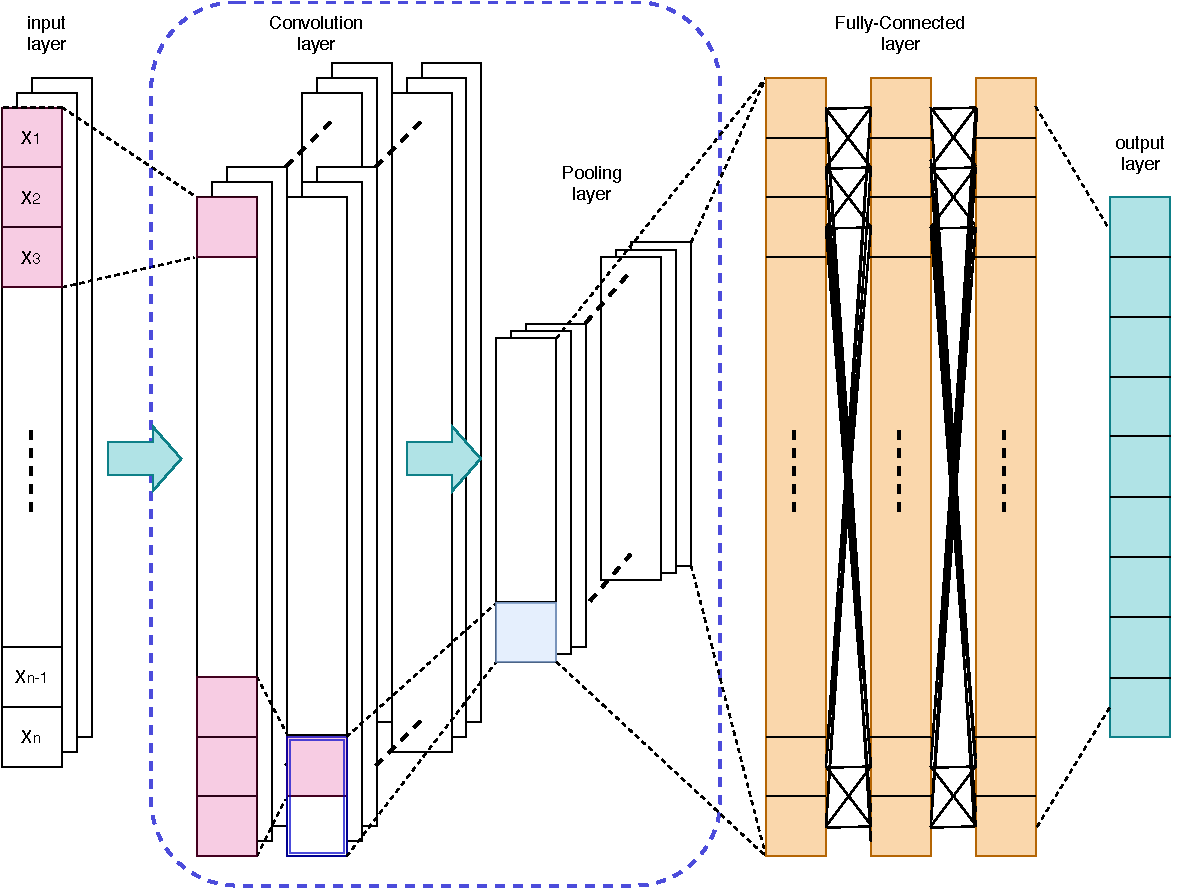
\includegraphics[width=12cm]{eps/cnn_architecture.pdf}
    \caption{CNNの基本構成}
    \label{fig:cnn_std}
   \end{center}
   \end{figure}
前述の Neocognitron 同様, 入力側に近い浅い層で特徴抽出を行うため, 畳み込みとプーリング処理を複数回行い特徴を計算する. 出力側に近い深い層で識別を行う. ネットワークの最終層では分類を行う各クラスごとの制度を算出するための出力層が追加される. 

\subsection{1次元の畳み込み処理}
畳み込み層がない従来のニューラルネットワークの場合, 入力の形式に問わず並列に扱ってしまう問題点がある. 例えば入力が画像である場合, あるピクセルと近傍のピクセル値は似た値になることが多く逆に離れた点同士には近傍のピクセルほどパターンや傾向を見いだせないことが多い. 時系列データの場合でも計測している事象が時間軸上で連続しており, 近傍点は似た値に, 離れた点はそうではない事が考えられる. このようにある一点において, 距離的に近いところとでなすはずの特徴を従来のニューラルネットワークでは捉えきれない可能性がある. 
前述の通り, 局所特徴量の抽出に優れた CNN の方が時系列データにおけるパターンに関する重要な特徴を捉えきれる可能性が高く有用だと考えた. 

畳み込み層で行う処理について説明する. 
畳み込み演算は入力データに対してフィルタ(カーネル)を適用する. 
本研究では入力データは1軸または3軸の時系列データであるため,  CNN の中でも1次元の畳み込み層を持つ 1D CNN を用いている. 
長さ$W$の1次元データに対する畳み込みを考える. 1つのデータ点をインデックス$i$を用いて$x_{i}$と表す. また同様に長さ$H$のフィルタ(カーネル)に対しても1つのフィルタ点をインデックス$p$を用いて$h_{p}$と表す. これらを積和演算することで畳み込み処理後のデータが得られる. 
\begin{equation}
{u_{i}=\sum_{p=0}^{H-1} x_{i+p} h_{p}}
\end{equation}

次にチャネルについて考える. 
チャネル番号$ k(= 0, 1, 2, 3, ..., K − 1)$とおく. 入力データが3軸である場合, チャネルはx, y, z軸方向データの K = 3と考えることができる. これを用い前述の式を拡張する. 
\begin{equation}
{u_{i}=\sum_{k=0}^{K-1}\sum_{p=0}^{H-1} x_{i+p,k} h_{pk}}
\end{equation}

次に畳み込み演算を行う層について考える. 
第 $l$ 層の畳込み層について, 前層$l − 1$ 層の出力$z^{(l-1)}_{ik}$に M 種類のフィルタ $h_{pkm}(m =
0, 1, 2, 3, ..., M − 1)$ を適用し, バイアス$ b_{m}$ を考慮するとフィルタからからの出力$u_{im}$は以下の式で定義される. 
\begin{equation}
{u_{im}=\sum_{k=0}^{K-1}\sum_{p=0}^{H-1} z^{(l-1)}_{i+p,k,m} h_{pkm}+b_{m}}
\end{equation}

活性化関数$f$を定義し, フィルタからの出力$u_{im}$をかけ合わせた畳み込み層の出力$z^{(l)}_{im}$を得る. 
\begin{equation}
{z^{(l)}_{im}=f(u_{im})}
\end{equation}

1次元畳み込み演算を以下の図\ref{fig:1dconv}に示す. 
\begin{figure}[H]
    \begin{center}
    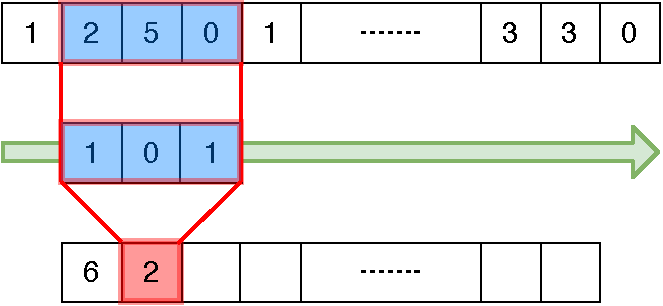
\includegraphics[width=12cm]{eps/1dconv.pdf}
    \caption{1次元畳み込み演算}
    \label{fig:1dconv}
   \end{center}
   \end{figure}

\subsection{1次元プーリング}
CNN において, プーリング層は畳み込み層と併せて使用される. 
主に畳み込み層で得た局所特徴に圧縮を行うような形で使用されることが多く, そのため畳み込み層の後層に配置される. 情報の圧縮を行う事により, フィルタ形状の位置ずれをある程度許容し, かつ計算量を抑えるという効果が期待できる. 
構造はシンプルであり, ある局所領域から代表値を抽出することで実現される. 
代表的な手法に局所領域中から最大値を取り出す最大プーリングが挙げられる. 

1次元最大プーリングを以下の図\ref{fig:1dpool}に示す. 

\begin{figure}[H]
    \begin{center}
    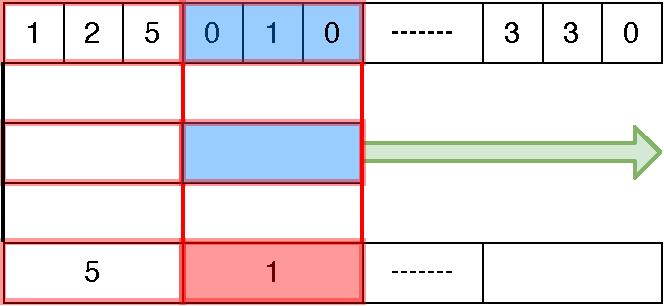
\includegraphics[width=12cm]{eps/1dpool.pdf}
    \caption{1次元最大プーリング処理}
    \label{fig:1dpool}
   \end{center}
   \end{figure}

% Local Variables:
% TeX-master: "main"
% mode: yatex
% End:
